\documentclass{standalone}
\usepackage{PhysicalChemistryNote}
\begin{document}
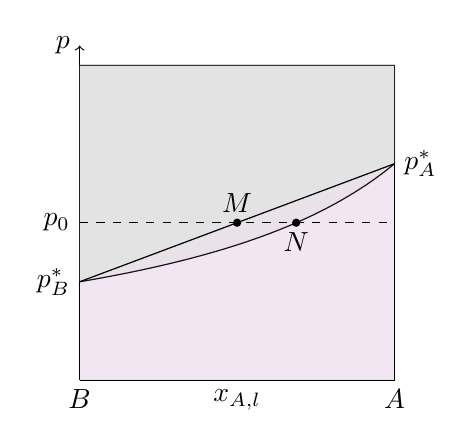
\begin{tikzpicture}
    \draw[-] (0,0) -- (4,0);
    \draw[->] (0,0) -- (0,4.25) node[left]{$p$};
    \draw[-] (4,0) -- (4,4);
    \draw[-] (0,4) -- (4,4);
    \node[below] at (0,0) {$B$};
    \node[below] at (4,0) {$A$};
    \node[below] at (2,0) {$x_{A,\l}$};
    \draw[domain=0:4] plot[smooth](\x,{4*1.25*2.75/(11-1.5*\x)});
    \filldraw[fill=lightgray,opacity=0.25,domain=0:4] plot[smooth](\x,{4*1.25*2.75/(11-1.5*\x)}) -- (4,4) -- (0,4);
    \filldraw[fill=violet,opacity=0.05,domain=0:4] plot[smooth](\x,{4*1.25*2.75/(11-1.5*\x)}) -- (4,0) -- (0,0);
    \filldraw[fill=lightgray,opacity=0.25] (0,1.25) -- (4,2.75) -- (4,4) -- (0,4);
    \filldraw[fill=violet,opacity=0.05] (0,1.25) -- (4,2.75) -- (4,0) -- (0,0);
    \node[left] at (0,1.25) {$p_B^\ast$};
    \node[left] at (0,2) {$p_0$};
    \node[right] at (4,2.75) {$p_A^\ast$};
    \draw[-] (0,1.25) -- (4,2.75);
    \draw[dashed] (0,2) -- (4,2);
    \fill (2,2) circle (1.5pt) node[above]{$M$};
    \fill (2.75,2) circle (1.5pt) node[below]{$N$};
    
\end{tikzpicture}
\end{document}